\documentclass{article}

\usepackage{array}
\usepackage{graphicx}

\begin{document}

\title{Hall Effect}
\author{GSI: Caleb Eades}
\date{11/8}
\maketitle

\section{The Hall Effect}

\subsection{Moving Slab}

A metal strip of length $L$ and width $w$ and thickness $t$ is moves with a velocity $v$ through a magnetic field $B_0$ into the page as shown below. If a potential difference of $V_0$ is measured between points a and b across the strip, calculate the speed $v$ of the strip.

\begin{figure}[h]
	\begin{center}
	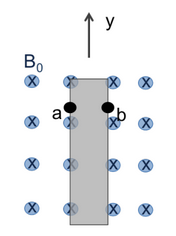
\includegraphics[width=0.2\textwidth]{Hall.png}
	\end{center}
\end{figure}

\textit{Source: modified from Halliday, Chapter 34-4, problem 39}

\subsection{Stationary Slab}

Suppose we have a rectangular block with length $l$, width $d$, and height $h$ in the $x$,$y$, and $z$ directions respectively. A current $\vec{I} = I \hat{x}$ flows through it. There is an external magnetic field $\vec{B} =  B \hat{y}$.
\begin{itemize}
	\item[(a)] Derive the Hall voltage $V_H$ for this setup.
	\item[(b)] Find an expression for the Hall constant 
	\[
	K_H = \frac{V_H}{B I}
	\]
	in terms of the charge carrier concentration $n$.
	\item[(c)] Using these results, how can you determine the sign and density of charge carriers in a material?
\end{itemize}

\textit{Source: Dan and Vetri}


\end{document}
